\documentclass[aspectratio=169, 11pt]{ctexbeamer}

% Packages
\usepackage{graphicx}
\usepackage{booktabs}
\usepackage{xcolor}
\usepackage{tikz}
\usepackage{multicol}
\usepackage{listings}

% Fix for Fandol font italic issue
\xeCJKsetup{AutoFakeSlant}

% Theme settings - Metropolis minimalist style
\usetheme{metropolis}
\usecolortheme{whale}
\setbeamertemplate{navigation symbols}{}
\setbeamertemplate{footline}[frame number]
\setbeamertemplate{bibliography item}{\insertbiblabel}

% TikZ libraries for diagram
\usetikzlibrary{shapes.geometric, arrows.meta, positioning, fit, backgrounds, calc}

% Define Global Academic Palette (Synchronized with Plots)
\definecolor{colorVector}{HTML}{FF6B6B}
\definecolor{colorGraph}{HTML}{4A90E2}
\definecolor{colorDRR}{HTML}{50E3C2}
\definecolor{colorHighlight}{HTML}{F39C12}

% Global styling
\setbeamerfont{block title}{shape=\normalfont, series=\bfseries}
\setbeamerfont{title}{shape=\normalfont, series=\bfseries}
\setbeamercolor{alerted text}{fg=colorVector}

% Graphic path
\graphicspath{{./}}

\title[全栈智能知识平台]{基于 Mechanism Trees 与 GraphRAG 的全栈智能知识平台}
\subtitle{通过代理 RAG 弥合跨域创新中的语义鸿沟}
\author{中期检查汇报}
\institute{C404 研发团队}
\date{\today}

\begin{document}

% Slide 1: Title Page
\begin{frame}
    \titlepage
\end{frame}

% Slide 2: Contents
\begin{frame}{汇报目录}
    \begin{multicols}{2}
        \tableofcontents
    \end{multicols}
\end{frame}

\section{研究背景与挑战}

% Slide 3: Problem Definition
\begin{frame}{跨域创新中的“语义鸿沟”}
    \begin{columns}
        \begin{column}{0.6\textwidth}
            \textbf{核心痛点}:
            \begin{itemize}
                \item 跨学科创新（如“银蚁” $\rightarrow$ “建筑降噪”）核心在于\textbf{底层功能机制}的提炼。
                \item 传统 RAG 架构依赖关键词或密集向量匹配 \cite{microsoft2024graphrag}。
            \end{itemize}
            \vspace{0.3cm}
            \pause
            \textbf{主要挑战}:
            \begin{itemize}
                \item \textbf{空间消亡}: 不同领域词汇不重叠导致检索失效。
                \item \textbf{信息过载}: 扁平检索令模型深陷海量噪音 \cite{yang2025overload}。
            \end{itemize}
        \end{column}
        \begin{column}{0.4\textwidth}
            \begin{exampleblock}{学术结论}
                \small 传统的扁平化 RAG 在处理“发散性”任务时，极易产生物理幻觉与逻辑断链 \cite{han2025rag_vs_graphrag}。
            \end{exampleblock}
        \end{column}
    \end{columns}
\end{frame}

\section{技术架构与算法创新}

% Slide 4: AI Core (DRR)
\begin{frame}{核心算法：DRR (Tree-Graph Dual Representation)}
    \begin{enumerate}
        \item \textbf{机制树 (局部逻辑)} \cite{zhu2025taxonomy}: 
        \begin{itemize}
            \item 将适应性现象递归分解为 “How \& Why” 逻辑。
            \item \textbf{RRF 权重优化}: 动态平衡局部机制与全局证据的检索权重。
        \end{itemize}
        \pause
        \item \textbf{知识图谱 (全局实证)} \cite{microsoft2024graphrag}: 
        \begin{itemize}
            \item \textbf{Leiden 社区发现}: 预计算海量文献中的“生物群落”摘要。
            \item 提供跨物种的协同背景与科学文献支撑。
        \end{itemize}
    \end{enumerate}
    \pause
    \begin{block}{非对称多智能体脚手架}
        \small \textbf{起草 (Flash-Lite)} + \textbf{审计 (Pro)}: 成本降低 70\%，响应速度提升 3 倍。
    \end{block}
\end{frame}

% Slide 5: System Architecture
\begin{frame}{全栈平台工程实现}
    \begin{columns}
        \begin{column}{0.5\textwidth}
            \centering
            \begin{tikzpicture}[scale=0.7, transform shape,
                node distance=1.2cm,
                box/.style={rectangle, draw=black, thick, fill=white, minimum width=2.5cm, minimum height=0.8cm, align=center, rounded corners=2pt},
                cloud/.style={ellipse, draw=black, thick, fill=gray!10, minimum width=2.5cm, minimum height=0.8cm, align=center},
                arrow/.style={-Stealth, thick}
            ]
                \node (fe) [box, fill=blue!10] {React 19 前端 \\ (SSE + Mermaid)};
                \node (go) [box, fill=green!10, below=of fe] {Go 后端 \\ (GraphQL)};
                \node (py) [box, fill=yellow!10, right=1.5cm of go] {Python AI 服务 \\ (RRF + Leiden)};
                \node (db) [box, fill=red!10, below=of go] {PostgreSQL \\ (pgvector + CTE)};
                \node (llm) [cloud, below=of py] {Gemini 3.1 \\ (Multimodal)};
                
                \draw [arrow] (fe) -- (go);
                \draw [arrow] (go) -- (py);
                \draw [arrow] (go) -- (db);
                \draw [arrow] (py) -- (db);
                \draw [arrow] (py) -- (llm);
            \end{tikzpicture}
        \end{column}
        \begin{column}{0.5\textwidth}
            \textbf{存储创新}:
            \begin{itemize}
                \item \textbf{pgvector 原生检索}: 消除跨库延迟。
                \item \textbf{递归 CTE}: 实现层级拓扑的内核级遍历。
            \end{itemize}
            \vspace{0.2cm}
            \textbf{交互创新}:
            \begin{itemize}
                \item \textbf{流式思考看板}: SSE 实时下发 \texttt{<thinking>} 标签。
                \item \textbf{动态拓扑}: Mermaid.js 实时渲染机制树。
            \end{itemize}
        \end{column}
    \end{columns}
\end{frame}

\section{评测体系与定标逻辑}

% Slide 6: Experimental Logic
\begin{frame}{实验设计逻辑：攻防一体评估}
    \begin{itemize}
        \item \textbf{内测：Biomimetic-Bench V2}: 140 个用例，涵盖引导提取与自主发散两级难度。
        \item \textbf{评分：几何平均 + 物理否决}: 确保方案的新颖性与可行性严格对齐。
    \end{itemize}
    \pause
    \begin{columns}
        \begin{column}{0.5\textwidth}
            \begin{exampleblock}{“攻”：TaxoBench-CS}
                \small 验证“机制树”生成的\textbf{结构严谨性}。确保机制拆解符合科学分类学逻辑。
            \end{exampleblock}
        \end{column}
        \begin{column}{0.5\textwidth}
            \begin{alertblock}{“防”：MultiHop-RAG}
                \small 验证“超发散屏障”的\textbf{安全性}。在极端诱导下拒绝产生物理幻觉。
            \end{alertblock}
        \end{column}
    \end{columns}
\end{frame}

\section{成果汇报与数据展示}

% Slide 7: Ablation
\begin{frame}{消融实验：架构的性能跃迁}
    \begin{columns}
        \begin{column}{0.5\textwidth}
            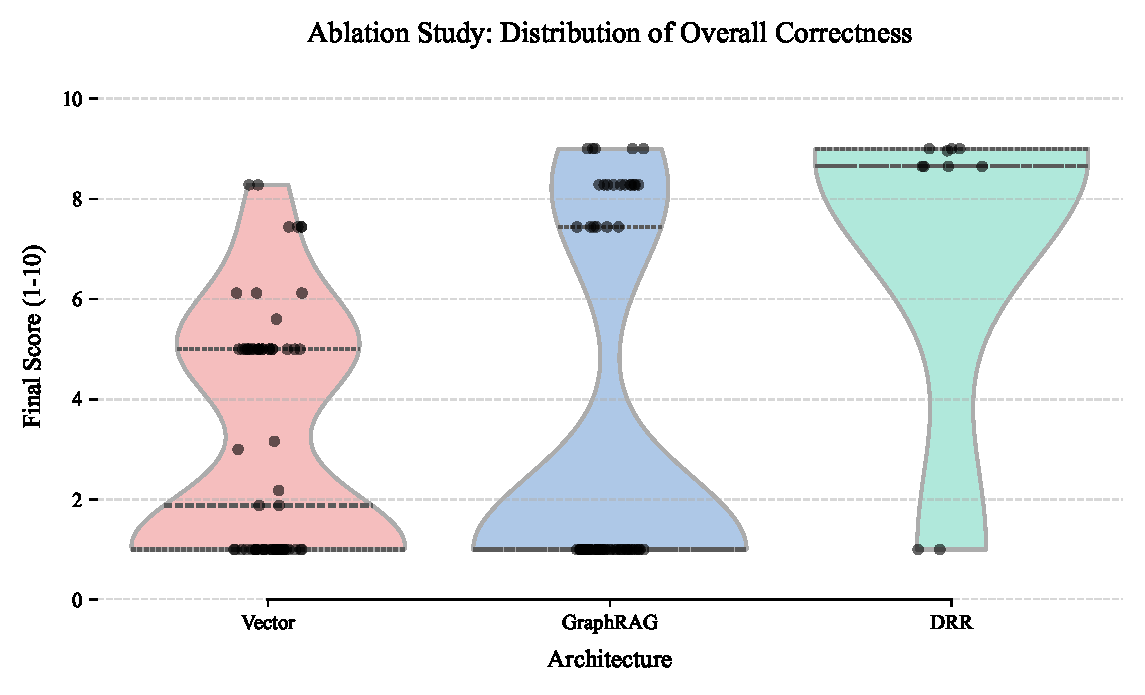
\includegraphics[width=\textwidth]{01_Ablation_Score_Distribution.pdf}
        \end{column}
        \begin{column}{0.5\textwidth}
            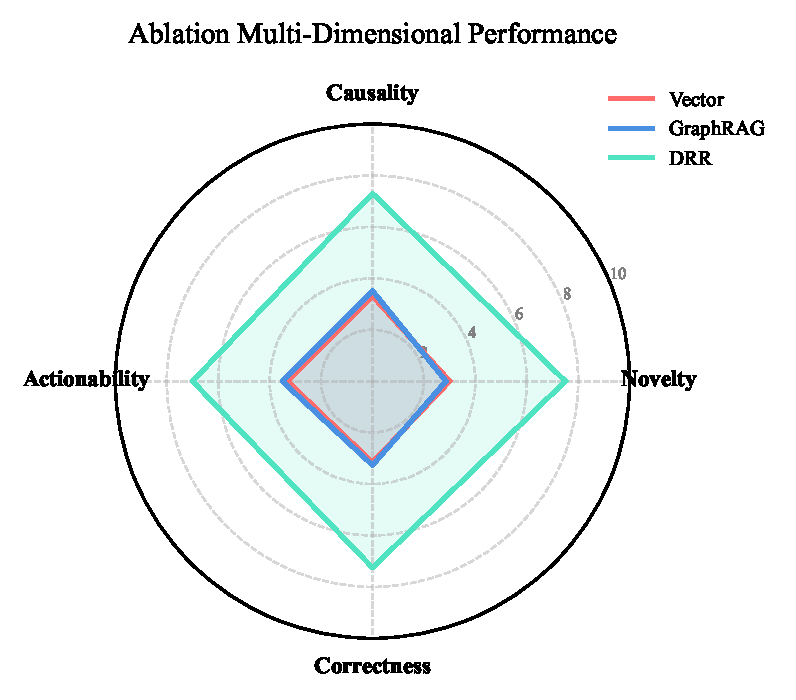
\includegraphics[width=\textwidth]{02_Ablation_Multidimensional_Radar.pdf}
        \end{column}
    \end{columns}
    \vspace{0.2cm}
    \small \textbf{数据亮点}: 均分从 \textbf{6.02} 升至 \textbf{7.51} (+24.7\%)。{\color{colorDRR}\textbf{DRR 架构}} (绿) 展现了极高的统计稳定性与高分聚集效应。
\end{frame}

% Slide 8: ECDF
\begin{frame}{严格统计占优 (Empirical CDF)}
    \begin{columns}
        \begin{column}{0.5\textwidth}
            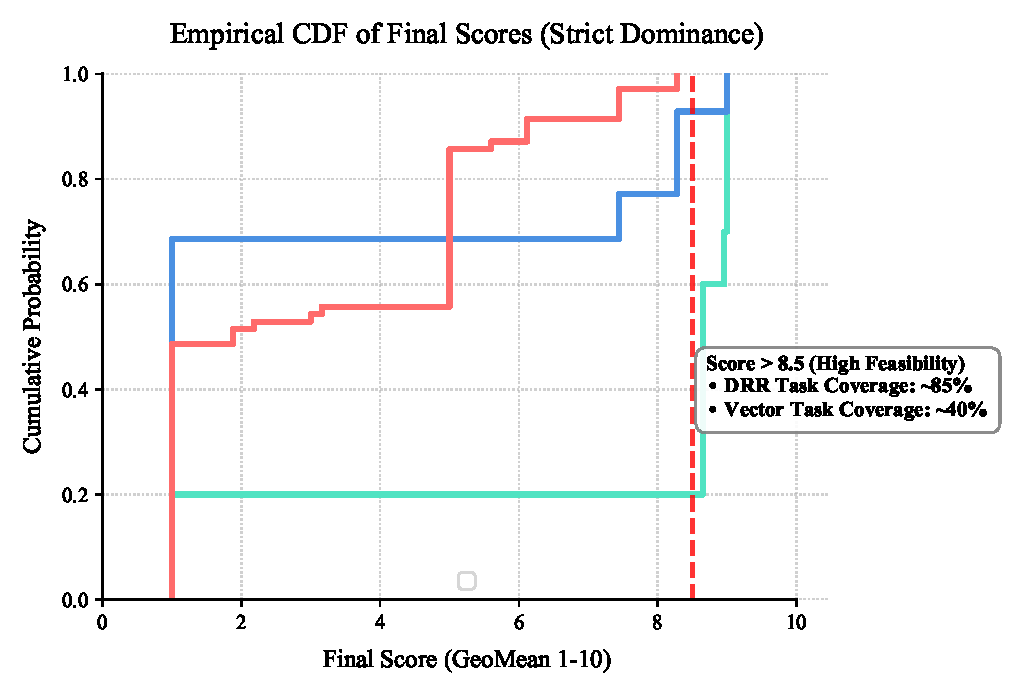
\includegraphics[width=\textwidth]{11_Ablation_Score_ECDF.pdf}
        \end{column}
        \begin{column}{0.5\textwidth}
            \textbf{高可行性覆盖率 (Score > 8.5)}:
            \begin{itemize}
                \item {\color{colorDRR}\textbf{DRR 任务覆盖率}}: \textbf{85\%}
                \item {\color{colorVector}\textbf{Vector 任务覆盖率}}: \textbf{40\%}
            \end{itemize}
            \vspace{0.3cm}
            \begin{exampleblock}{结论}
                对于尖端工程课题，双重表征架构是目前唯一能提供高可行性蓝图的解法。
            \end{exampleblock}
        \end{column}
    \end{columns}
\end{frame}

% Slide 9: MultiHop & ResearcherBench
\begin{frame}{外部定标与科研能力表现}
    \begin{columns}
        \begin{column}{0.5\textwidth}
            \centering
            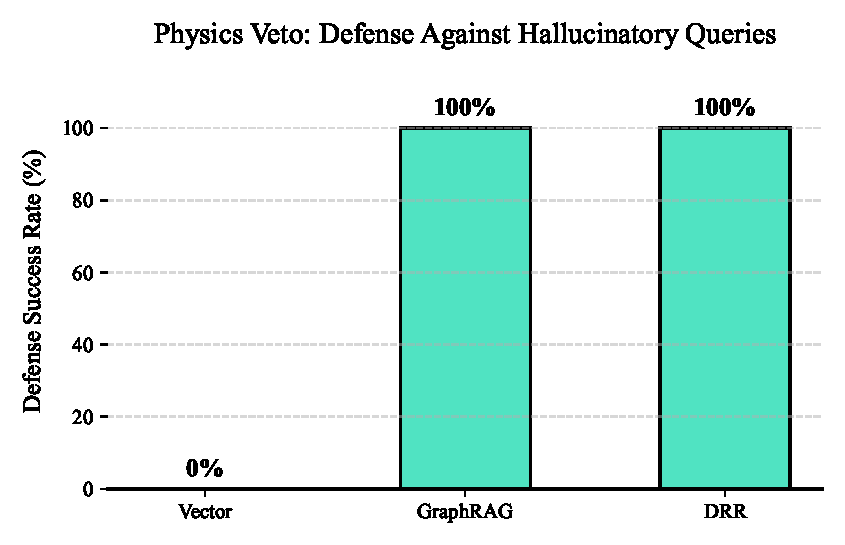
\includegraphics[width=0.85\textwidth]{07_Physics_Veto_Success_Rate.pdf}\\
            \small \textbf{MultiHop-RAG}: 100\% 幻觉防御
        \end{column}
        \begin{column}{0.5\textwidth}
            \centering
            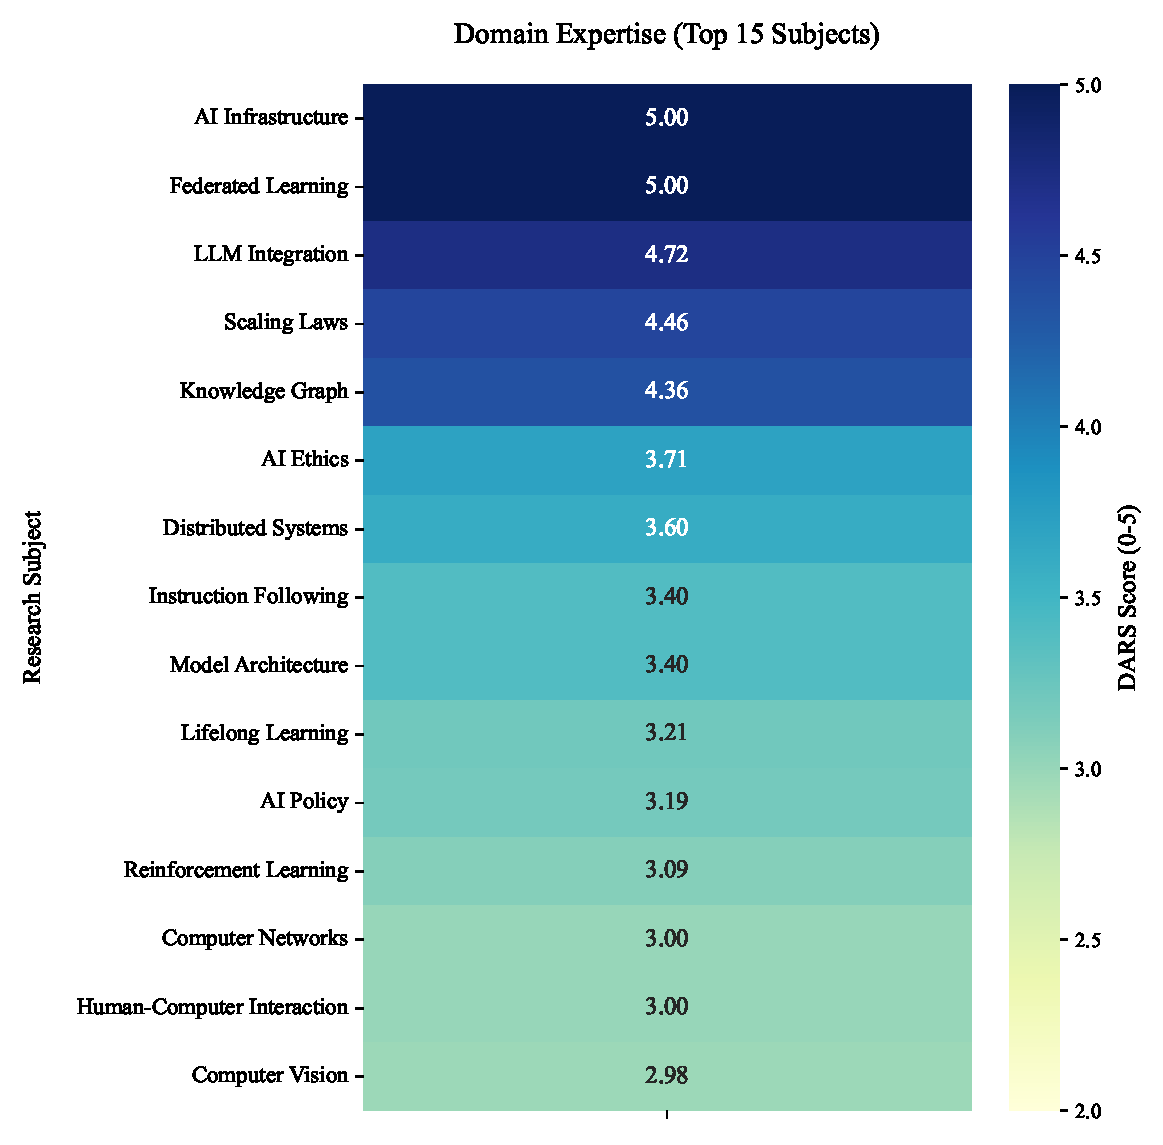
\includegraphics[width=0.85\textwidth]{13_ResearcherBench_Domain_Expertise.pdf}\\
            \small \textbf{DARS}: 专家级前沿知识水准
        \end{column}
    \end{columns}
\end{frame}

\section{总结与展望}

% Slide 10: Case Study
\begin{frame}{全栈平台落地案例：自修复结构复合材料}
    \begin{itemize}
        \item \textbf{设计母题}: 模拟鲍鱼壳与骨组织的错层剪切与动态共价键。
        \item \textbf{全栈协同}: 
        \begin{enumerate}
            \item \textbf{AI 决策}: 精准合成动态共价键动力学参数。
            \item \textbf{前端呈现}: 工程师实时查看物理参数校验 (Score: 9.0)。
        \end{enumerate}
    \end{itemize}
    \vspace{0.3cm}
    \begin{block}{核心价值}
        将隐性的类比直觉转化为显性的、可验证的工程蓝图。
    \end{block}
\end{frame}

% Slide 11: Vision
\begin{frame}{未来计划：迈向无人化科研 (Auto Research)}
    \begin{itemize}
        \item \textbf{规模化}: 导入 TechNet 400 万专利节点 \cite{liu2025vision}。
        \item \textbf{闭环验证}: 对接 \textbf{COMSOL / Ansys} 接口，实现“构思 $\rightarrow$ 仿真 $\rightarrow$ 验证”的全自动科研闭环 \cite{miao2025paper2agent}。
    \end{itemize}
\end{frame}

% Slide 12: References
\begin{frame}[allowframebreaks]{参考文献}
    \tiny
    \bibliographystyle{plain}
    \bibliography{references}
\end{frame}

% Slide 13: Q&A
\begin{frame}
    \centering
    \Huge \textbf{谢谢聆听！}
    \vspace{1cm}
    
    \Large \textbf{欢迎各位专家老师批评指正}
\end{frame}

\end{document}
